\documentclass{IEEEcsmag}

\usepackage[colorlinks,urlcolor=blue,linkcolor=blue,citecolor=blue]{hyperref}
\expandafter\def\expandafter\UrlBreaks\expandafter{\UrlBreaks\do\/\do\*\do\-\do\~\do\'\do\"\do\-}
\usepackage{upmath,color}

\usepackage[spanish]{babel}
%\usepackage[latin1]{inputenc}
\usepackage[utf8]{inputenc}  

\jvol{1}
\jnum{1}
\paper{1}
\jmonth{Noviembre}
\jname{ITICs letters}
\jtitle{Proyectos Integradores}
\pubyear{2023}
\usepackage{cite}
\usepackage{amsmath,amssymb,amsfonts}
\usepackage{algorithmic}
\usepackage{graphicx}
\usepackage{textcomp}
\usepackage{xcolor}
\usepackage{listings}

\newtheorem{theorem}{Theorem}
\newtheorem{lemma}{Lemma}


\setcounter{secnumdepth}{0}

\begin{document}

%imprimir código
\lstnewenvironment{javaCode}[1][]
{\lstset{
    language=Java,
    basicstyle=\scriptsize\ttfamily,
    numbers=none, % Modificado: quitar los números de línea
    keywordstyle=\color{blue},
    commentstyle=\color{gray},
    stringstyle=\color{purple},
    breaklines=true,
    breakatwhitespace=true,
    tabsize=4,
    showspaces=false,
    showstringspaces=false,
    frame=single,
    captionpos=b,
    floatplacement=!h,
    #1
}}
{}


\sptitle{Proyecto Integrador de Primer Semestre}

\title{Software de resolución de problemas de Ingeniería }

\author{Chávez Atanacio Yael Antonio}
\affil{Instituto Tecnológico Superior del Occidente del Estado de Hidalgo, Mixquiahuala, Hgo., 42700, Mexico}

\author{Neri Pérez Giovany Humberto}
\affil{Instituto Tecnológico Superior del Occidente del Estado de Hidalgo, Mixquiahuala, Hgo., 42700, Mexico}

%\author{Third Author III}
%\affil{Institute, City, (State), Postal Code, Country}

\markboth{ITSOEH/ITICS/PROYECTO INTEGRADOR PRIMER SEMESTRE}{THEME/FEATURE/DEPARTMENT}

\begin{abstract}
Un resumen (abstract) es un párrafo único que resume los aspectos importantes del manuscrito. A menudo indica si el manuscrito es un informe de un trabajo nuevo, una revisión o una descripción general, o una combinación de ambos. No cite referencias en el resumen. Este tipo de documento debe incluir contenido propiedad de los autores; es decir, no debe contener contenido de otras fuentes, ademas la redacción debe  estar dirigida a un tipo de lector técnico general. Este archivo se encuentra disponible en \href{https://github.com/fcuadrosgithub/integrador-primero.git}{https://github.com/fcuadrosgithub/integrador-primero.git}.
\end{abstract}

\maketitle
\chapteri{L}a introducción debe proporcionar información general (incluidas referencias relevantes) y debe indicar el propósito del manuscrito. En esta sección describa de manera clara y precisa el objetivo del proyecto integrador, la metodología que piensa usar y los resultados obtenidos de manera muy general. Dentro de esta sección puede citar trabajos relevantes de otros si lo cree necesario.

Esta sección debe dar un panorama muy general al lector de cual es el problema a resolver, que metodología utilizó para dar solución al problema y cuales fueron los resultados obtenidos. 

La redacción del manuscrito debe ser en tercera persona y queda estrictamente prohibido el uso de palabras coloquiales o Español informal. En lugar de esto utilice un lenguaje formal que el mayor numero de personas pueda entender.
\clearpage

\section{Resolución Problema 1} 

\subsection{\textbf{Descripción del problema:}}
En el contexto de geometría analítica, la tarea es obtener la ecuación de la recta que pasa por los puntos $A$ y $B$, así como determinar el ángulo interno $\alpha$ que se forma entre la recta y el eje horizontal. Por lo tanto la solución implica el uso de conceptos trigonométricos y algebraicos para abordar este problema geométrico de manera eficiente.

\subsection{\textbf{Definición de solución:}}
La solución propuesta emplea tres funciones matemáticas clave. Primero, se calcula la inclinación de la recta mediante la función \texttt{inclinación}, luego se determina la intersección en el eje $Y$ con la función \texttt{intersección}, y finalmente se calcula el ángulo interno $\alpha$ con la función \texttt{ángulo}. Estas funciones trabajan en conjunto para proporcionar la ecuación de la recta y el ángulo deseado.

\subsection{\textbf{Diseño de la solución:}}
Para el diseño de la solución observamos en la ecuación de la recta, si dos puntos distintos $P(x_{1}, y_{1})$ y $Q(x_{2}, y_{2})$ se ubican en la curva $y=f(x)$, la pendiente de la recta secante que une los dos puntos es:
\begin{equation}
    m_{sec}=\frac{y_{2} - y_{1}}{x_{2} - x_{1}} = \frac{f_{(x2)} - f_{(x1)} }{x_{2} - x_{1}}/
    \label{eqn:rectaPendiente}
\end{equation}

La forma punto-pendiente de la ecuación de la recta, con una coordenada especifica en el plano cartesiano se define como:
\begin{equation}
    b = y_{1} - m * x_{1}
     \label{eqn:eqnRecta}

\end{equation}
\begin{figure}[H]
    \centering
    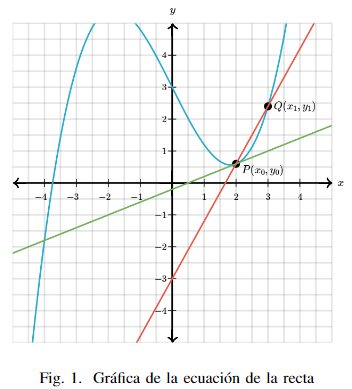
\includegraphics[width = 6 cm]{Latex-imágenes/GraficaEcuación.png}
    \caption{Gráfica de la ecuación de la recta}
    \label{fig:GraficaEcuacionRecta}
\end{figure}

Utilizando este método, es posible encontrar la ecuación de la recta a partir de dos puntos. Recordando que si los dos puntos son idénticos la recta será una linea vertical.

El algoritmo de solución para encontrar la ecuación de la recta pendiente  (ec. \ref{eqn:rectaPendiente}) comienza solicitando al usuario dos puntos $P(x_{1}, y_{1})$ y $Q(x_{2}, y_{2})$.\\

\centering
\begin{figure}[H]
    \centering
    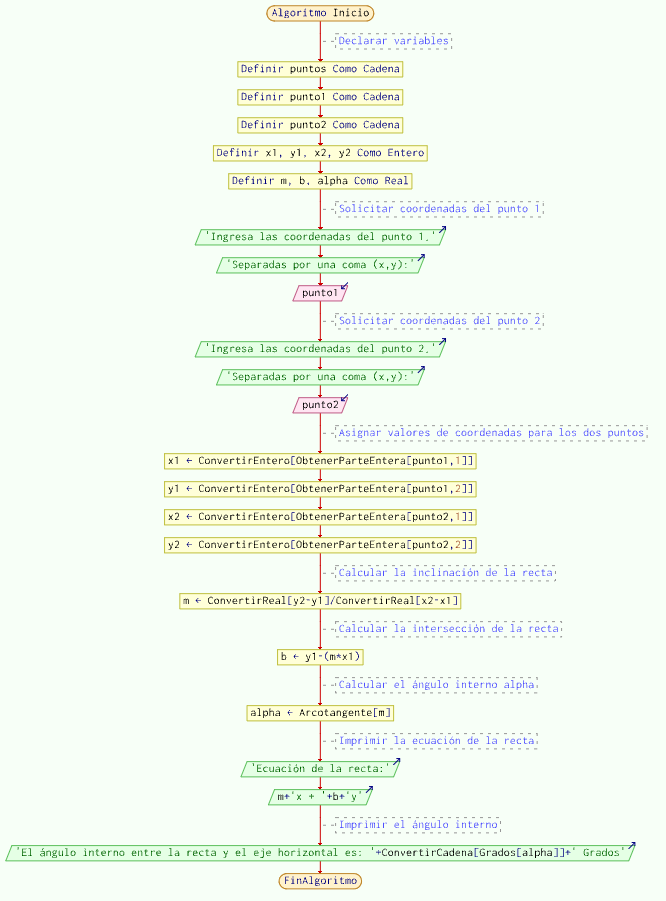
\includegraphics[width = 6 cm]{Latex-imágenes/Diagrama.png}
    \caption{Diagrama de flujo usado.}
\end{figure}


\subsection{\textbf{Desarrollo de la solución:}}
En el primer fragmento, se solicitan las coordenadas de dos puntos, A y B, que se ingresan en formato (x, y). Las coordenadas se leen como cadenas para separar las componentes x e y. Finalmente, se cierra el objeto Scanner para liberar los recursos.

\begin{javaCode}

Scanner puntos = new Scanner (System.in);
        
    //Solicitar puntos para la ecuacion de la recta  
    System.out.println("""
                        Ingresa las coordenadas del punto 1.
                        seperadas por una coma (x,y):
                           """);
    
    String[] punto1 =puntos.nextLine().split(",");
        
    System.out.println("""
                        Ingresa las coordenadas del punto 1.
                        seperadas por una coma (x,y):
                        """);
    
    String[] punto2 =puntos.nextLine().split(",");
        
    //cerrar el escaneo
    puntos.close();
        
\end{javaCode}

Las coordenadas separadas se convierten de cadenas a números enteros utilizando Integer.parseInt(). El método trim() se utiliza para eliminar cualquier espacio en blanco que pueda haber alrededor de las coordenadas.

\begin{javaCode}
    //Asignar valor de coordenadas a x,y para dos puntos
    int x1= Integer.parseInt(punto1[0].trim());
    int y1= Integer.parseInt(punto1[1].trim());
       
    int x2= Integer.parseInt(punto2[0].trim());
    int y2= Integer.parseInt(punto2[1].trim());
\end{javaCode}

Aquí se calcula la pendiente ($m$) de la recta utilizando la fórmula
\[
m = \frac{{y_2 - y_1}}{{x_2 - x_1}}
\]
y luego se calcula la intersección en el eje $Y$ ($b$) utilizando la fórmula.(ec. \ref{eqn:eqnRecta})
La ecuación de la recta resultante es\\ $y = mx + b$.

\begin{javaCode}
    //Calculo para la inclinacion de la recta  
    Double m = (double)(y2 - y1)/(x2 - x1);
       
    //Calcular Interseccion de la recta
    Double b= y1 -(m * x1);
\end{javaCode}
Se calcula el ángulo interno (\(\alpha\)) entre la recta y el eje horizontal utilizando la función \texttt{Math.atan(m)}. El resultado se convierte de radianes a grados.\\
\begin{javaCode}
    // Calcular el ángulo interno $\alpha$
        Double alpha = Math.atan(m);
        
\end{javaCode}
Finalmente, se imprime la ecuación de la recta y el ángulo interno en grados. La ecuación se imprime en formato \(mx + by\), y el ángulo se imprime en grados.
\begin{javaCode}
   //Imprimir ecuacion de la recta
        
        System.out.println("Ecuacion de la recta igual= \n" +
                 m + " x + " + b + " y ");
       //Imprimir el resultado de el ángulo interno 
        System.out.println("El ángulo interno entre la recta y el eje horizontal es: " 
                + String.format("%.3f", Math.toDegrees(alpha)) + " Grados");
                
\end{javaCode}
La función String.format() formatea un número decimal según el formato especificado en la cadena de formato.(En este caso 3f es el formato que indica que el número debe redondearse a tres). decimales
\subsection{\textbf{Depuración y pruebas:}}
\begin{tabular}{|c|c|c|c|c|c|}
    \hline
    \textbf{Punto1} & \textbf{Punto2} & \textbf{ (\(m\))} & \textbf{(\(b\))} & \textbf{ (\(\alpha\))} & \textbf{Recta} \\
    \hline
    (-1, 0) & (2, -3) & -1.0 & 1.0 & -45.000 & \(y = -x + 1\) \\
    \hline
    (-4, 1) & (1, 4) & 0.6 & 3.4 & 30.964 & \(y = -x + 5\) \\
    \hline
    (3, -2) & (0, 1) & -1.0 & 3.0 & -54.738 & \(y = -x + 1\) \\
    \hline
    % Pruebas necesarias
\end{tabular}
\caption{Pruebas para el programa de ecuación de la recta}
\label{tab:pruebas}
\end{table}
\clearpage

\section{Resolución Problema 2} 
Dada una ecuación cuadrática regresar los valores de las raíces, en caso de que estén sobre el conjunto de números reales, en caso contrario indicar que la solución esta en el conjunto de los números complejos.


\subsection{\textbf{Descripción del problema:}}
El problema planteado se centra en la resolución de una ecuación cuadrática y la determinación de sus posibles soluciones. La ecuación cuadrática tiene la forma general $ax^{2}+bx+c$, donde a, b y c son los coeficientes dados. El objetivo es aplicar la fórmula general:
\begin{equation}
\\
\\ x = \frac{{-b \pm \sqrt{{b^2 - 4ac}}}}{{2a}} \\
\end{equation}
\\
\\Para obtener las soluciones de la ecuación.

Para determinar la naturaleza de las soluciones, se utiliza el discriminante, que está dado por la expresión 
\begin{equation}
 b^2 - 4ac 
\end{equation}
\\Dependiendo del valor del discriminante, se obtienen tres casos posibles:
\begin{itemize}
    \item Si el discriminante > 0 se dan dos soluciones
    \item Si el discriminante = 0 se da una solución
    \item Si el discriminante es < 0 la solución se encuentra en el conjunto de los números complejos. 
\end{itemize}
 Estos casos permiten clasificar las soluciones de la ecuación cuadrática en función de su naturaleza y son determinantes para comprender las propiedades y características de la ecuación en cuestión.


\begin{figure}[H]
    \centering
    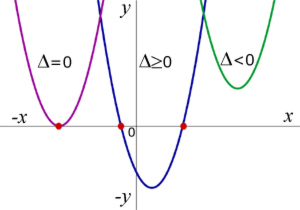
\includegraphics[width = 6 cm]{Latex-imágenes/discriminant.jpg}
    \caption{Discriminante}
    \label{fig:Discriminante}
\end{figure}


\subsection{\textbf{Definición de solución:}}
Se plantea la resolución de una ecuación cuadrática en la forma 
\begin{equation}
ax^{2}+bx+c
\end{equation}
donde se procede al cálculo del discriminante y a la evaluación de tres condiciones. En caso de que el discriminante sea mayor que cero, se llevan a cabo dos operaciones y se presenta el resultado correspondiente. Si el discriminante es igual a cero, se realiza una operación y se muestra el resultado obtenido. Por otro lado, si el discriminante resulta ser negativo, se informa al usuario que la ecuación en cuestión no cuenta con soluciones reales.

Acto seguido se muestra el diagrama de flujo, el cual es la base del programa.

\begin{figure}[H]
    \centering
    \includegraphics[width = 6 cm]{Latex-imágenes//Diagrama2.png}
    \caption{Diagrama de flujo}
    \label{fig:diagrama de flujo}
\end{figure}


\subsection{\textbf{Diseño de la solución:}}
Se plantea la resolución de una ecuación cuadrática en la forma 
\begin{equation}
ax^{2}+bx+c
\end{equation}
donde se procede al cálculo del discriminante y a la evaluación de tres condiciones. En caso de que el discriminante sea mayor que cero, se llevan a cabo dos operaciones y se presenta el resultado correspondiente. Si el discriminante es igual a cero, se realiza una operación y se muestra el resultado obtenido. Por otro lado, si el discriminante resulta ser negativo, se informa al usuario que la ecuación en cuestión no cuenta con soluciones reales.

Acto seguido se muestra el diagrama de flujo, el cual es la base del programa.

\begin{figure}[H]
    \centering
    \includegraphics[width = 6 cm]{LaTeX/imagenes/Diagrama2.png}
    \caption{Diagrama de flujo}
    \label{fig:diagrama de flujo}
\end{figure}


\subsection{\textbf{Desarrollo de la solución:}}
eguidamente se mostrara el programa de java, donde se trabajo con la formula general. Para ello, se ocupan las librería Math y el objeto Scanner.
\begin{javaCode}
    
import java.util.Scanner;

    
        Crear un objeto Scanner para leer la entrada del usuario
        \begin{javaCode}
        Scanner coeficiente = new Scanner(System.in);
        \end{javaCode}
        Solicitar al usuario que ingrese el valor de A
        \begin{javaCode}
        System.out.println("Estimado usuario, por favor ingrese el valor de A: ");
        double a = coeficiente.nextDouble();
        \end{javaCode}
        Solicitar al usuario que ingrese el valor de B
        \begin{javaCode}
        System.out.println("Estimado usuario, por favor ingrese el valor de B: ");
        double b = coeficiente.nextDouble();
        \end{javaCode}
        Solicitar al usuario que ingrese el valor de C
        \begin{javaCode}
        System.out.println("Estimado usuario, por favor ingrese el valor de C: ");
        double c = coeficiente.nextDouble();
        \end{javaCode}
        Cierra el objeto Scanner
        \begin{javaCode}
        coeficiente.close();
        \end{javaCode}
        Calcula el discriminante de la ecuación cuadrática
        \begin{javaCode}
        double discriminante = b * b - 4 * a * c;
        \end{javaCode}
       El objetivo es verificar si el discriminante de una ecuación cuadrática es mayor que cero. Si se cumple esta condición, se determina que la ecuación tiene dos soluciones. Luego, se resuelven las soluciones y se muestra el resultado al usuario.
        \begin{javaCode}
        if (discriminante > 0) {
            double x1 = (-b + Math.sqrt(discriminante)) / (2 * a);
            double x2 = (-b - Math.sqrt(discriminante)) / (2 * a);
       
            System.out.println("Las soluciones son x1 = " + x1 + " y x2 = " + x2);
        }
        \end{javaCode}
        Verificar si el discriminante es igual a 0, si cumple con la condición, realiza la operación donde solo existe una única solución y la muestra al usuario
        \begin{javaCode}
        else if (discriminante == 0) 
           
            double x = -b / (2 * a);

            System.out.println("La solucion es: " + x);
        
        \end{javaCode}
        En caso de que el discriminante sea negativo, se determina que la ecuación cuadrática no tiene soluciones reales. Esta información se comunica al usuario.
        \begin{javaCode}
        else {
            System.out.println("no cuenta con soluciones reales.");
        }
    



\end{javaCode}



\subsection{\textbf{Depuración y pruebas:}}
del mismo. Donde se muestra los diferentes resultados posibles.
\begin{center}
\begin{tabular}{|c|c|c|c|c|}
\hline
No. & A & B & C & Resultado \\
\hline
1 & 19 & 17 & 18 & no cuenta con soluciones reales. \\
\hline
2 & 10 & 15 & 5 & La solución es:$x_1 = -0.5$ y $x_2=-1.0$ \\
\hline
3 & 1 & -2 & 1 & La solución es:$x=1 \\
\hline
4 & 2 & 4 & -6 &La solución es:$x_1 = 1.0$ y $x_2=-3.0$ \\
\hline
5 & 1 & 1 & 1 & No cuenta con soluciones reales. \\
\hline
\end{tabular}
\label{fig: Tabla de ejecución}
\end{center}
\clearpage

\section{Resolución Problema 3}
Dada una circunferencia con centro en el punto
C con coordenadas (x1, y1) y radio r, evaluar si
un punto T con coordenadas (x2, y2) esta dentro
del área de la circunferencia.


\subsection{\textbf{Descripción del problema:}}
El problema implica calcular la distancia de dos puntos 
Dónde el punto C y el punto T pueden ser definidos en el plano cartesiano (X,Y) y R es definidas asía los cuatro ejes, además debemos tomar en cuenta que el punto T se puede encontrar dentro o fuera de la circunferencia 


\subsection{\textbf{Definición de solución:}}
En el primer segmento considerando las variables X1,X2 y Y1,Y2 se plantea la siguiente solución se emplea la formula: distancia:
\\
${Distancia} = \sqrt{{(x_2 - x_1)^2 + (y_2 - y_1)^2}}$,
\\
Con esta formula se calcula la distancia entre los dos puntos  \texttt{(C y T)}.Posterior mente se verifica que el radio ingresado sea positivo, en dado caso de que el radio sea negativo se utilizara la formula: Radio*-1; con esta formula se convierte el radio negativo a positivo,finalmente verificamos que el punto se encuentre dentro de la circunferencia utilizando el radio . 
\\
-Observamos como se plasma en el plano cartesiano utilizando la formula de la distancia
\begin{figure}[H]
    \centering
    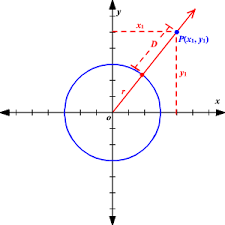
\includegraphics[width = 5 cm]{LaTeX/latex-imagenes/Imagen7.png}
    \caption{Gráfica del programa}
    \label{fig:imagen7}
\end{figure}


\subsection{\textbf{Diseño de la solución:}}
\begin{enumerate}[label=\textbf{\arabic*.}]

  \item Considerando las variables X,Y de cada punto calcula la distancia entre los dos puntos utilizando la siguiente formula: {distancia} = \sqrt{{(x_2 - x_1)^2 + (y_2 - y_1)^2}}.

  \item  Considerando que la variable r sea positiva se procedera al siguiente paso, de lo contrario se aplicara la siguiente ecuacion r*-1.
  \item considerando que la distancia sea menor al radio se puede decir que el punto T se encuentra dentro de la circunferencia, de lo contrario se considera que el punto se encuentra fuera de la circunferencia. 
  \\
  A continuación veremos el diagrama de flujo que fue la base para el desarrollo del programa.
\end{enumerate}
\begin{figure}[H]
    \centering
    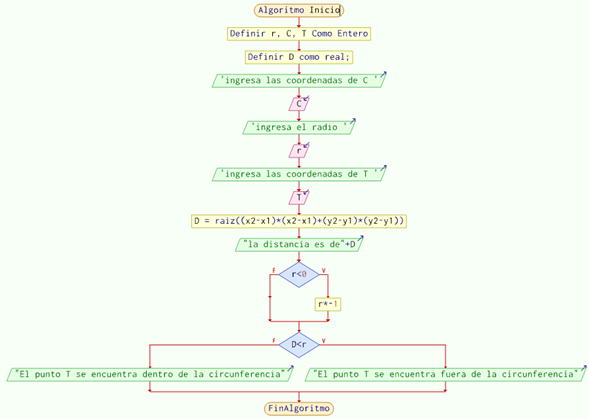
\includegraphics[width = 8 cm]{LaTeX/latex-imagenes/diagramaz.png}
    \caption{Diseño del programa}
    \label{fig:imagen7}
\end{figure}


\subsection{\textbf{Desarrollo de la solución:}}
A continuación, se muestra el código en Java para calcular la distancia entre dos puntos y verificar si se encuentran dentro de una circunferencia:


  \\
  \\
  
        Primero se solicita al usuario las coordenadas del punto C (x1,y1)
       \begin{javaCode}
        Scanner dato = new Scanner(System.in);
        System.out.print("Ingrese las coordenada del punto C primero x1: ");
        int x1 = dato.nextInt();
        System.out.print("Ingrese las coordenada del punto C despues  y1: ");
        int y1 = dato.nextInt();
         \end{javaCode}
         se solicita el radio de la circunferencia
       
        \begin{javaCode}
        System.out.println("Ingrese el radio de la circunferencia: ");
        int radio = dato.nextInt();
         \end{javaCode}
         
        solicitamos al usuario las coordenadas del punto T (x2,y2)
       \begin{javaCode}
        System.out.print("Ingrese las coordenada del punto T X2: ");
        int x2 = dato.nextInt();
        System.out.print("Ingrese las coordenada del punto T Y2: ");
        int y2 = dato.nextInt();
        \end{javaCode}
         Se realiza el cálculo  la distancia entre el punto C y el punto T con ayuda de la formula antes mencionada.
        \begin{javaCode}
        double distancia = Math.sqrt((x2 - x1) * (x2 - x1) + (y2 - y1) * (y2 - y1));
        \end{javaCode}
         Se imprime el resultado del calculo de la distancia.
          \begin{javaCode}
         System.out.println("la distancia es de "+distancia);
          \end{javaCode}
       
        Se verifica si el radio es positivo o negativo, si es negativo lo pasamos a positivo
         \begin{javaCode}
        int radio2=radio*-1;
\end{javaCode}
         Se calcula, si la distancia resulta menor o igual al radio entonces el punto T se encontrara dentro de la circunferencia, de lo contrario el punto T se encontrara fuera de la circunferencia .    
       
        \begin{javaCode}
                    if(radio<0){
            
        
        int radio2=radio*-1;
        if (distancia <= radio2) {
            System.out.println("El punto T está dentro de la circunferencia");
        } else {
            System.out.println("El punto T no está dentro de la circunferencia");
        }
        }
        
       if(radio>0){
           
       
            if (distancia <= radio) {
            System.out.println("El punto T está dentro de la circunferencia");
        } else {
            System.out.println("El punto T no está dentro de la circunferencia");
        }
    }
    
    
    }
    
}
    \end{javaCode}

    
\subsection{\textbf{Depuración y pruebas:}}
Se realizaron 5 pruebas al programa para validar su funcionamiento, a continuación veremos los siguientes resultados 



   \begin{figure}[H]
    \centering
    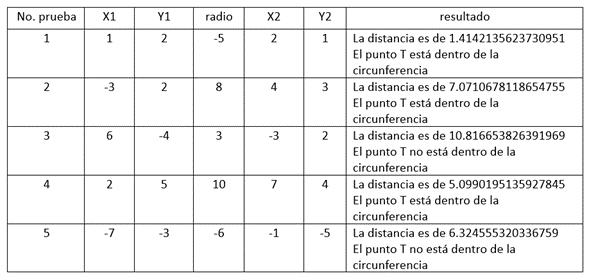
\includegraphics[width = 11 cm]{LaTeX/latex-imagenes/tabla de pruebas.png}
    \caption{Tabla de pruebas}
    \label{fig:Grafica de la distancia de dos puntos }
\end{figure}
\clearpage

\section{Resolución Problema 4}

\subsection{\textbf{Descripción del problema:}}

\subsection{\textbf{Definición de solución:}}

\subsection{\textbf{Diseño de la solución:}}

\subsection{\textbf{Desarrollo de la solución:}}

\subsection{\textbf{Depuración y pruebas:}}
\clearpage

\section{Resolución Problema 5}
Dado un numero binario de $n$ bits regresa su equivalente a decimal.


\subsection{\textbf{Descripción del problema:}}

Dar como resultante un numero binario.

\subsection{\textbf{Definición de solución:}}
La solución para convertir un número binario de n bits a su equivalente en decimal consiste en recorrer cada bit del número binario, multiplicar su valor por 2 elevado a la potencia correspondiente según su posición, y sumar los resultados. Al finalizar el recorrido, el valor obtenido será el equivalente decimal del número binario. Es importante verificar la validez del número binario y asegurarse de que esté compuesto únicamente por 0 y 1. El resultado se muestra como el equivalente decimal del número binario.


\subsection{\textbf{Diseño de la solución:}}
El programa solicita al usuario que ingrese un número binario de n bits. Se asegura de que el número ingresado consista únicamente en dígitos binarios 0 y 1. Si se detecta algún dígito decimal, el programa no funcionará.

Luego, se realiza la conversión del número binario ingresado a su equivalente decimal utilizando la fórmula de posición y peso explicada anteriormente.

Finalmente, el programa imprime el resultado de la conversión, es decir, el número decimal equivalente al número binario ingresado por el usuario.


\begin{figure}[H]
    \centering
    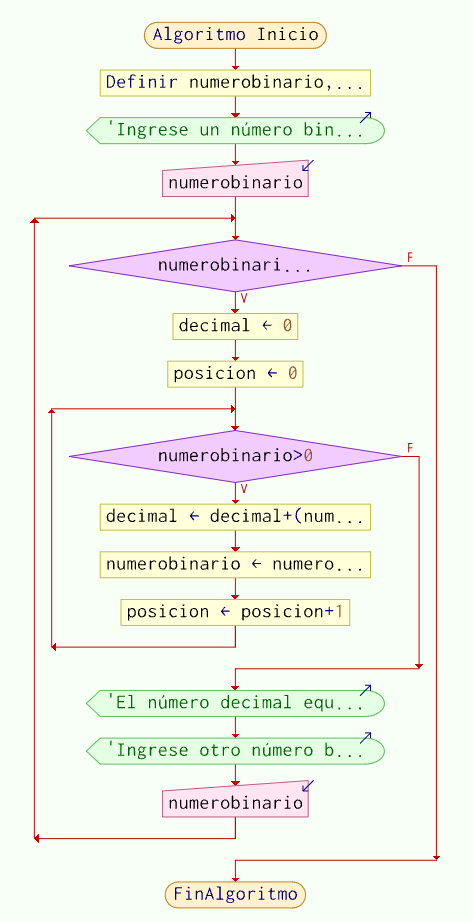
\includegraphics[width=6cm]{Latex-imágenes/ALGORITMO.png}
    \caption{Diagrama de flujo usado como base .}
\end{figure}


\subsection{\textbf{Desarrollo de la solución:}}
El desarrollo del código del programa en Java para la conversión de números binarios a decimales:

\begin{lstlisting}[style=javaStyle]
import java.util.Scanner;
import java.math.BigInteger;

public class NewClass {
    public static void main(String[] args) {
        Scanner bin = new Scanner(System.in);
        boolean continuar = true;
\end{lstlisting}
En esta paso en el programa son colocadas las variables $Scanner$ $BigInteger$
las cuales ayudaran al correr el programa

Se solicita al usuario ingresar un numero binario
\begin{lstlisting}[style=javaStyle]
// Bucle que permite al usuario ingresar números binarios hasta que ingrese 'x'

        while (continuar) {
        
            System.out.print("Ingrese un número en binario (o 'x' para terminar ): ")
            
            String entrada = bin.nextLine();
\end{lstlisting}

 La variable $while$ es utilizada como un "mientras" esta mantiene un bucle regresando a pedirnos un numero binario para su conversión a binario

\begin{lstlisting}[style=javaStyle]
                 // Si se ingresa 'x', el bucle se detiene;
            if (entrada.equalsIgnoreCase("x")) {
                continuar = false;
                continue;
            }
\end{lstlisting}

En esta línea, se declara una variable llamada decimal del tipo BigInteger. Se utiliza para almacenar el valor decimal resultante después de convertir el número binario ingresado. La función convertirBinarioADecimal se llama con el argumento entrada, que es el número binario ingresado por el usuario.

\begin{lstlisting}[style=javaStyle]
 // llama al método convertirBinarioADecimal para convertir el número binario ingresado a decimal
 
            BigInteger decimal = convertirBinarioADecimal(entrada);
            
\end{lstlisting}

 Esta línea imprime en la consola el mensaje "El número en decimal es: " seguido del valor almacenado en la variable decimal. Es decir, muestra el resultado de la conversión en formato decimal.

\begin{lstlisting}[style=javaStyle]
System.out.println("El número en decimal es: " + decimal);

\end{lstlisting}

Estas líneas definen el método convertirBinarioADecimal, que toma un argumento de tipo String llamado binario. El método crea un nuevo objeto BigInteger utilizando el constructor que toma dos argumentos: el número binario (binario) y la base (2) que se utiliza para interpretar el número binario y convertirlo a decimal. 

\begin{lstlisting}[style=javaStyle]
lic static BigInteger convertirBinarioADecimal(String binario) {
        return new BigInteger(binario, 2);

\end{lstlisting}

\text La fórmula se basa en el hecho de que cada posición en un número binario representa una potencia de 2. El dígito en la posición más a la derecha tiene un peso de \(2^0\), el siguiente dígito tiene un peso de \(2^1\), el siguiente tiene un peso de \(2^2\), y así sucesivamente.
\space

\begin{equation}

M = D0 * 2^0 + D1 * 2^1 + D2 * 2^2

\end{equation}


\subsection{\textbf{Depuración y pruebas:}}
En esta tabla se dasarrollan una seria de pruebas, 
\begin{figure}[H]
    \centering
    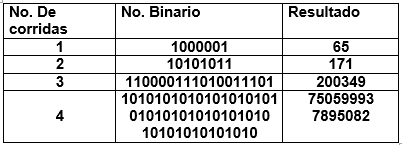
\includegraphics[width=10cm]{Latex-imágenes/TABLA DE PRUEBAS.png}
    \caption{Prueba de escritorio.}
\end{figure}

\clearpage

\section{Resolución Problema 6}

\subsection{\textbf{Descripción del problema:}}

\subsection{\textbf{Definición de solución:}}

\subsection{\textbf{Diseño de la solución:}}

\subsection{\textbf{Desarrollo de la solución:}}

\subsection{\textbf{Depuración y pruebas:}}
\clearpage


\section{CONCLUSION}
El manuscrito debe incluir direcciones futuras de la investigación. Se recomienda encarecidamente a los autores que no hagan referencia a varias figuras o tablas en la conclusión; estos deben mencionarse en el cuerpo del artículo.
\vspace*{-8pt}


\section{AGRADECIMIENTOS}
Esta sección es opcional. Si los autores creen necesario agradecer a alguien por haber aportado al desarrollo de su proyecto integrador de alguna u otra forma, esta sección esta destinada para esto.


\def\refname{REFERENCES}

\begin{thebibliography}{1}

\bibitem{AA1}
G. M. Amdahl, G. A. Blaauw, and F. P. Brooks, ``Architecture of the IBM System/360,'' {\it IBM J. Res. Dev}., vol. 8, no. 2, pp. 87--101, 1964. (Journal)

\bibitem{BB1}
IBM Corporation, IBM Knowledge Center - IBM Secure Service Container (Secure Service Container). [Online]. Available: {https://www.ibm.com/support/\break knowledgecenter/en/HW11R/com.ibm.hwmca.kc\_se.doc/\break introductiontotheconsole/wn2131zaci.html} (URL)

\bibitem{CC1}
J. Williams, ``Narrow-band analyzer,'' Ph.D. dissertation, Dept.  Elect. Eng., Harvard Univ., Cambridge, MA, USA, 1993. (Thesis or dissertation)

\bibitem{DD1}
J. M. P\'erez, R. Berlanga, M. J. Aramburu, and T. B. Pedersen, ``Integrating data warehouses with web data: A survey,'' {\it IEEE Trans. Knowl. Data Eng}., early access, Dec. 21, 2007, doi:10.1109/TKDE.2007.190746. (Preprint)

\bibitem{EE1}
W.-K. Chen, {\it Linear Networks and Systems}. Belmont, CA, USA: Wadsworth,  1993, pp. 123--135. (Book)

\bibitem{FF1}
S. P. Bingulac, ``On the compatibility of adaptive controllers,'' in {\it Proc. 4th Ann. Allerton Conf. Circuits Syst. Theory}, 1994,  pp. 8--16. (Conference proceedings)

\bibitem{GG1}
K. Elissa, ``An overview of decision theory,'' unpublished. (Unpublished manuscript)

\bibitem{HH1}
R. Nicole, ``The last word on decision theory,'' {\it J. Comput. Vis.}, submitted for publication. (Pending publication)

\bibitem{II1}
C. J. Smith and J. S. Smith, Rocky Mountain Research Laboratories, Boulder, CO, USA, private communication, 1992. (Private communication)
\end{thebibliography}\vspace*{-8pt}


\begin{IEEEbiography}{Cuadros Romero Francisco Javier}{\,}Todas las biografías se limitan a un párrafo y deben ser muy sintéticas. Se puede agregar la carrera en la cual el estudiante esta enrolado. Se pueden mencionar los 3 intereses principales del estudiante. Asi como su aspiración en el corto y mediano plazo. Al final de la biografia de cada estudiante se debe agregar el enlace a su pagina personal en Github: 
%\vadjust{\vfill\pagebreak}
\end{IEEEbiography}

\begin{IEEEbiography}{Neri Pérez Giovany Humberto}{\,}es un estudiante de la ingeniería en Tecnologías de la Información y Comunicaciones con una pasión desbordante por los videojuegos, el anime y los ``corridos tumbados''. Nacido y criado en  Tetepango, desde temprana edad mostró un gran interés por la tecnología y los avances en el campo de la informática. Aunque sus intereses pueden parecer diversos, Giovany encuentra inspiración en la creatividad y la narrativa tanto de los videojuegos como del anime. Estos medios le han enseñado la importancia de la perseverancia, la resolución de problemas y el trabajo en equipo. El objetivo principal de Giovany es completar sus estudios universitarios en ITICs, con especialización en ciberseguridad. Sueña con trabajar en el campo de la ciberseguridad, protegiendo sistemas e información vital de ataques cibernéticos y contribuyendo así a la seguridad digital de las organizaciones.
\end{IEEEbiography}

\end{document}

